% Introduction part 

\section{LoRa Radio Frequency Fingerprinting Identification}

\subsection{LoRa}
\begin{frame}
  \frametitle{What is LoRa}
    LoRa is a radio frequency communication technology with an emphasis on:
    \begin{enumerate}
      \item Long Range (up to 5km)
      \item Low power consumption (in milliwatts)
      \item Low transmission rate (in kbps)
    \end{enumerate}

    With such features, LoRa is widely used in the communication of isolated sensors.  
    % take the example of the CO2 sensors 
\end{frame}

\begin{frame}
  \frametitle{Some words on LoRaWan}
  \begin{figure}
    \begin{center}
      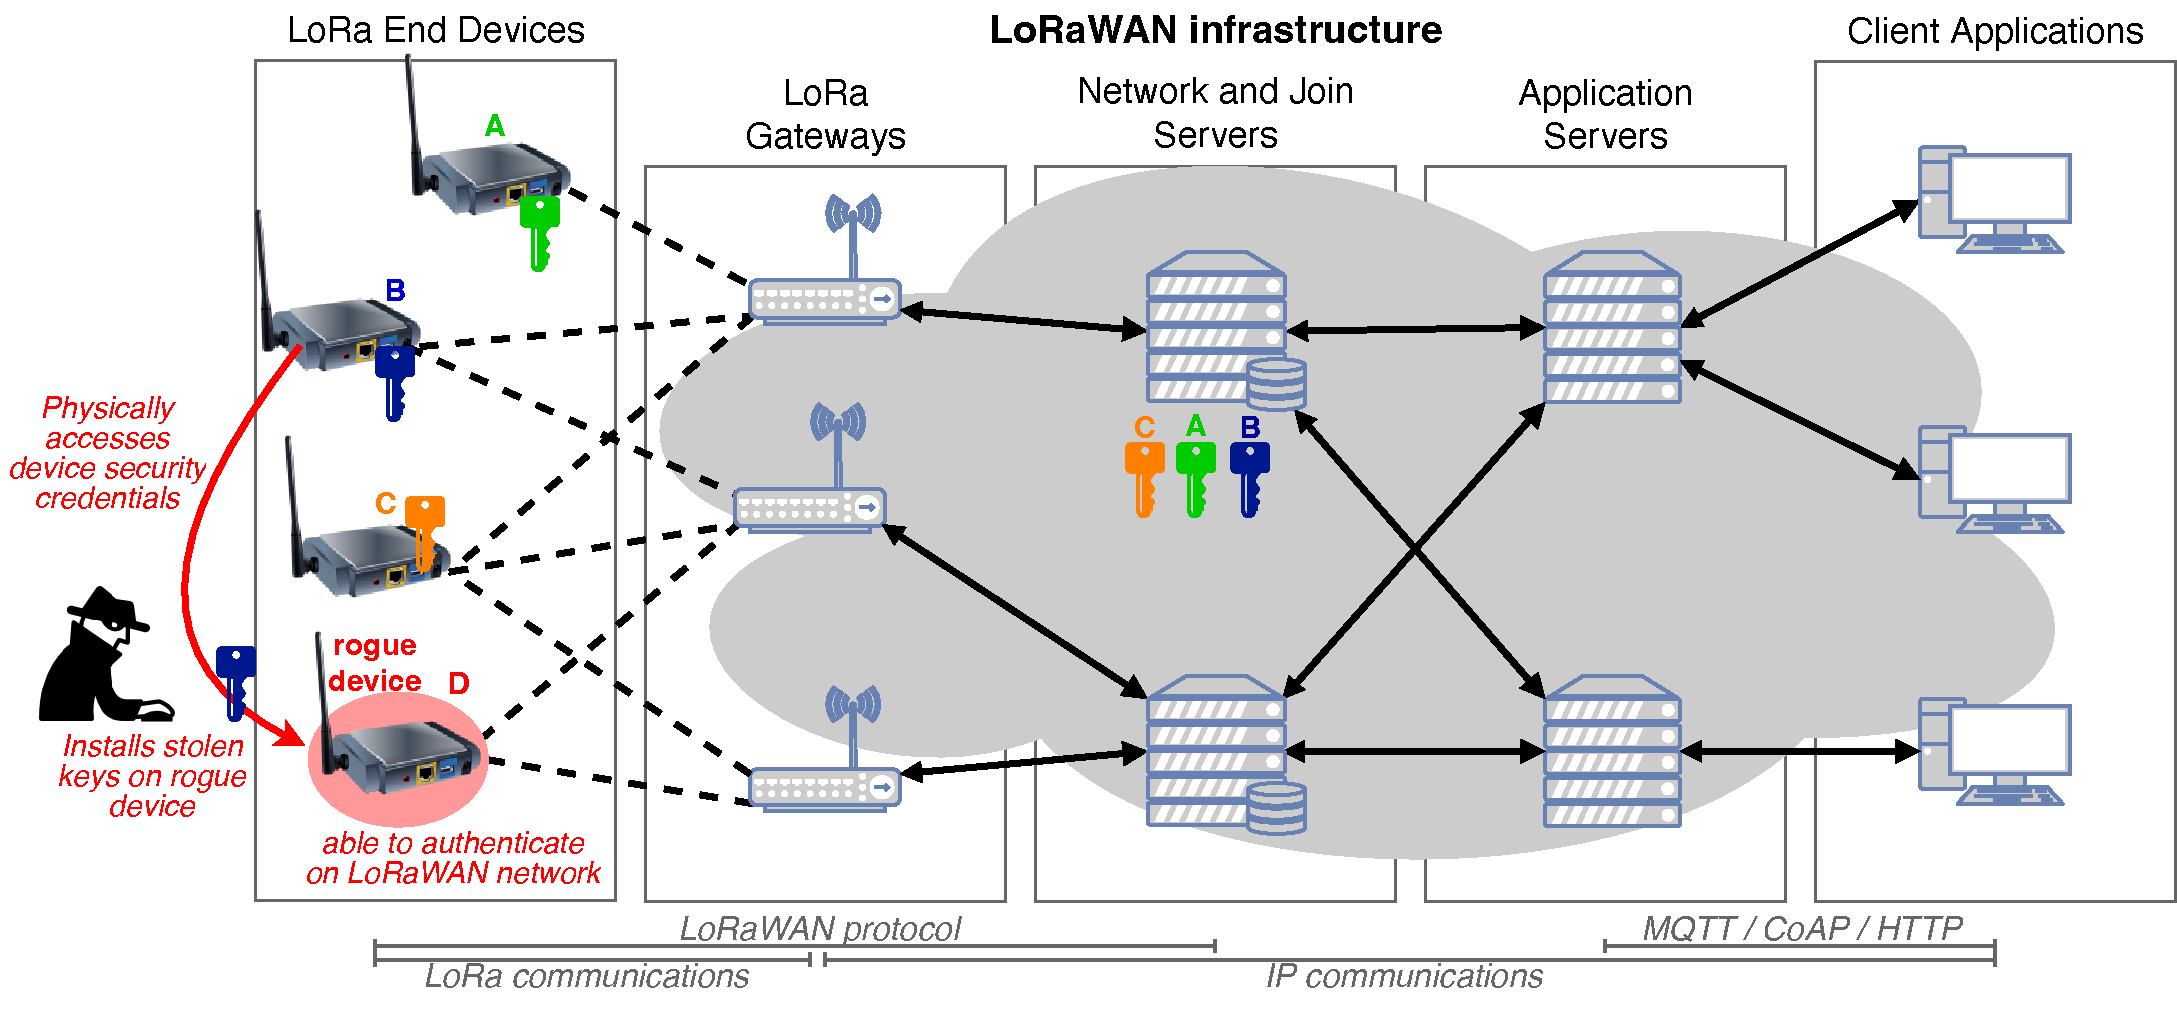
\includegraphics[width=0.95\textwidth]{figures/LoRaWAN2.pdf}
    \end{center}
  \end{figure}
\end{frame}

\begin{frame}
  \frametitle{LoRa physical layer}
  \small
  LoRa physical layer is based on Chirp Spread Spectrum (CSS) modulation. 


  \begin{definition}[Chirp Spread Spectrum modulation]
    CSS modulation is based on sine signals whose frequency varies linearly over time.
  \end{definition}

  \begin{figure}
    \begin{center}
      \includesvg[width=0.95\textwidth]{figures/timeVsFreq.svg}
    \end{center}
    \caption{Time vs Frequency Domain of a LoRa up-chirp}
  \end{figure}
\end{frame}

\begin{frame}
  \frametitle{LoRa frame}

  The LoRa frame is composed of :
  \begin{enumerate}
    \item A preamble (8 up-chirps and Sync word)
    \item A Start of Frame Delimiter (SFD)
    \item A payload
  \end{enumerate}

  \begin{figure}
    \begin{center}
      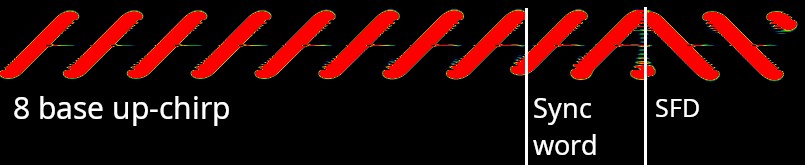
\includegraphics[width=0.95\textwidth]{figures/LoRaPreambleWithText.png}
    \end{center}
    \caption{Preamble and SFD parts on a spectrogram}
  \end{figure}
\end{frame}


\subsection{Radio frequency fingerprinting identification}
\begin{frame}
  \frametitle{RFFI}
  \begin{definition}{Radio Frequency Fingerprints (RFF)}
    are subtle impairments in a device transmission due to its hardware components. 
 \end{definition}
 \pause

 RFF are unique to each device which makes it a key candidate for device authentication.
  
 \pause

  \begin{definition}{Radio Frequency Fingerprinting Identification (RFFI)}
    bases Identification on the RFF of a device. 
 \end{definition}

\end{frame}

\subsection{State of the art}
\begin{frame}
  \frametitle{State of the art}
  Recent studies\footnotemark  have looked into LoRa RFFI with DL models.

  However, as stated by Aqeel in a recent survey\footnotemark , only four datasets are publicly available. 
  \begin{enumerate}
    \item Zenodo 
    \item Oregon state University cloud 
    \item IEEE dataport (2)  
  \end{enumerate}


  \footnotetext[1]{\cite{shen2021radio} and \cite{al2021deeplora}}
  \footnotetext[2]{\cite{AqeelSurvey}}


\end{frame}

\subsection{Objective}
\begin{frame}
  \frametitle{Objective}
  
  The Goals of this internship were to:
  \begin{enumerate}
      \item Understand the principles of LoRa technology
      \item Establish a test bed scenario to collect LoRa radio frequency signals
      \item Collect LoRa RF signals at different distances to evaluate the impact on DL classification
  \end{enumerate}
  
\end{frame}


%%%%%%%%%%%%%%%%%%%%%%%%%%%%%%%%%%%%%%%%%%%%
% appendix
